% ----------------------------------------------------------------------
% Set the document class
% ----------------------------------------------------------------------
\documentclass[12pt]{article}

% ----------------------------------------------------------------------
% Define external packages, language, margins, fonts, new commands 
% and colors
% ----------------------------------------------------------------------
\usepackage[utf8]{inputenc} % Codification
\usepackage{listings}
\usepackage[english]{babel} % Writing idiom
\usepackage{stackengine}
\usepackage[export]{adjustbox} % Align images
\usepackage{amsmath} % Extra commands for math mode
\usepackage{amssymb} % Mathematical symbols
\usepackage{amsthm}
\usepackage{anysize} % Personalize margins
    \marginsize{2cm}{2cm}{2cm}{2cm} % {left}{right}{above}{below}
\usepackage{appendix} % Appendices
\usepackage{cancel} % Expression cancellation
\usepackage{caption} % Figure numeration
\usepackage{cite} % Citations, like [1 - 3]
\usepackage{color} % Text coloring
\usepackage{fancyhdr} % Head note and footnote
    \pagestyle{fancy}
    \fancyhf{}
    \fancyhead[L]{\footnotesize IST} % Left of Head note
    \fancyhead[R]{\footnotesize ULisboa} % Right of Head note
    %\fancyfoot[L]{\footnotesize Course} % Left of Footnote
    \fancyfoot[C]{\thepage} % Center of Footnote
    %\fancyfoot[R]{\footnotesize Degree} % Right of Footnote
    \renewcommand{\footrulewidth}{0.4pt} % Footnote rule
\usepackage{float} % Utilization of [H] in figures
\usepackage{graphicx} % Figures in LaTeX
\usepackage[colorlinks = true, plainpages = true, linkcolor = istblue, urlcolor = istblue, citecolor = istblue, anchorcolor = istblue]{hyperref}
\usepackage{indentfirst} % First paragraph
\usepackage{siunitx} % SI units
\usepackage{subfigure} % Subfigures

% Random text (not needed)
\usepackage{lipsum}
\usepackage{duckuments}

\definecolor{mygreen}{rgb}{0,0.6,0}
\definecolor{mygray}{rgb}{0.5,0.5,0.5}
\definecolor{mymauve}{rgb}{0.58,0,0.82}

\lstset{ %
  backgroundcolor=\color{white},   % choose the background color
  basicstyle=\footnotesize,        % size of fonts used for the code
  breaklines=true,                 % automatic line breaking only at whitespace
  captionpos=b,                    % sets the caption-position to bottom
  commentstyle=\color{mygreen},    % comment style
  escapeinside={\%*}{*)},          % if you want to add LaTeX within your code
  keywordstyle=\color{blue},       % keyword style
  stringstyle=\color{mymauve},     % string literal style
}


% New and re-newcommands
\newcommand{\sen}{\operatorname{\sen}} % Sine function definition
\newcommand{\HRule}{\rule{\linewidth}{0.5mm}} % Specific rule definition
\renewcommand{\appendixpagename}{\LARGE Appendices}

% Colors
\definecolor{istblue}{RGB}{3, 171, 230}
\definecolor{dkgreen}{rgb}{0,0.6,0}
\definecolor{gray}{rgb}{0.5,0.5,0.5}

\DeclareMathOperator*{\minimize}{minimize}

%%%%%%%%%%%%%%%%%%%%%%%%%%%%%%%%%%%%%%%%%%%%%%%%%%%%%%%%%%%%%%%%%%%%%%%%
%                                 Document                             %
%%%%%%%%%%%%%%%%%%%%%%%%%%%%%%%%%%%%%%%%%%%%%%%%%%%%%%%%%%%%%%%%%%%%%%%%
\begin{document}

% ----------------------------------------------------------------------
% Cover
% ----------------------------------------------------------------------
\begin{center}
    \begin{figure}
        \vspace{-1.0cm}
        
\includegraphics[scale = 0.3, left]{Images/IST_A.eps} % IST logo
    \end{figure}
    \mbox{}\\[2.0cm]
    \textsc{\Huge Optimization and Algorithms Project}\\[2.5cm]
    %\textsc{\LARGE Degree}\\[2.0cm]
    %\HRule\\[0.4cm]
    %{\large \bf Title -- Report Template IST [\texttt{EN}]}\\[0.2cm]
    %\HRule\\[1.5cm]
\end{center}

\begin{flushleft}
    \textbf{Authors:}
\end{flushleft}

\begin{center}
    \begin{minipage}{0.5\textwidth}
        \begin{flushleft}
            Duarte Calado de Almeida (95565)\\
            Francisco Manuel Leal Mithá Ribeiro (95578)\\
            José Pedro Baptista de Figueiredo (96259) \\
            João De Assis Marcos Soares Nabais (97349)\\ 
        \end{flushleft}
    \end{minipage}%
\end{center}
    
\begin{flushleft}
    \large $\boxed{\text{\bf Group} \ 8}$\\[4.0cm]
\end{flushleft}
    
\begin{center}
    \large \bf 2022/2023 -- 1º Semester, P1
\end{center}

\thispagestyle{empty}

\setcounter{page}{0}

\newpage

% ----------------------------------------------------------------------
% Contents
% ----------------------------------------------------------------------
\tableofcontents 

\newpage

% ----------------------------------------------------------------------
% Body
% ----------------------------------------------------------------------
\section{Task 1}

\begin{figure}[H]
    \centering
    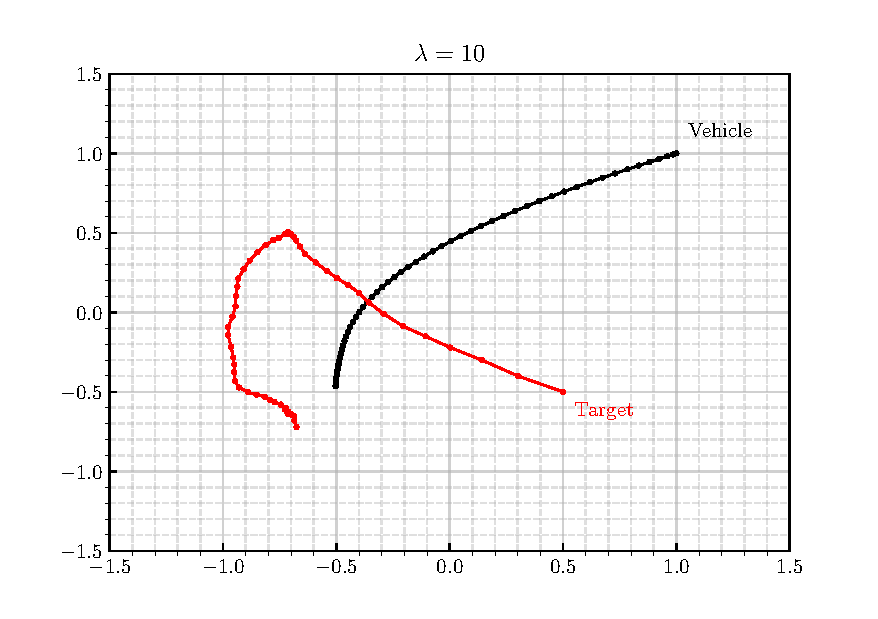
\includegraphics{../../src/task_1/output/ex_1_i=1.pdf}
\end{figure}

\begin{figure}[H]
    \centering
    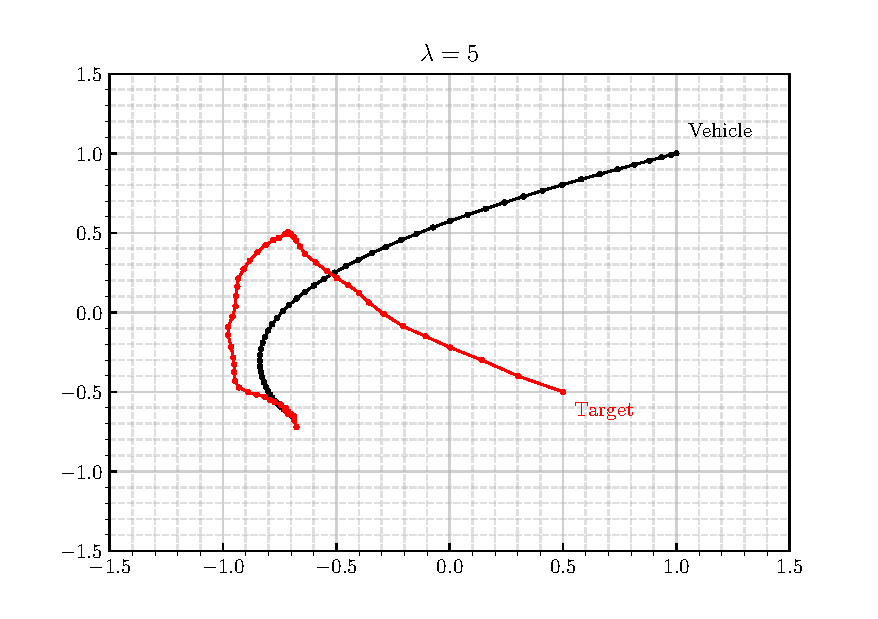
\includegraphics{../../src/task_1/output/ex_1_i=2.pdf}
\end{figure}

\begin{figure}[H]
    \centering
    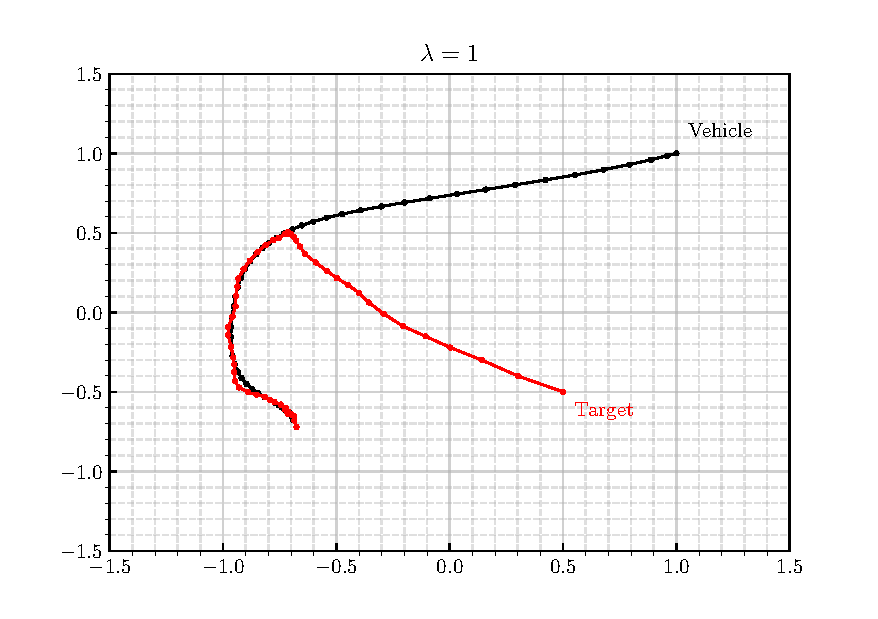
\includegraphics{../../src/task_1/output/ex_1_i=3.pdf}
\end{figure}

\begin{figure}[H]
    \centering
    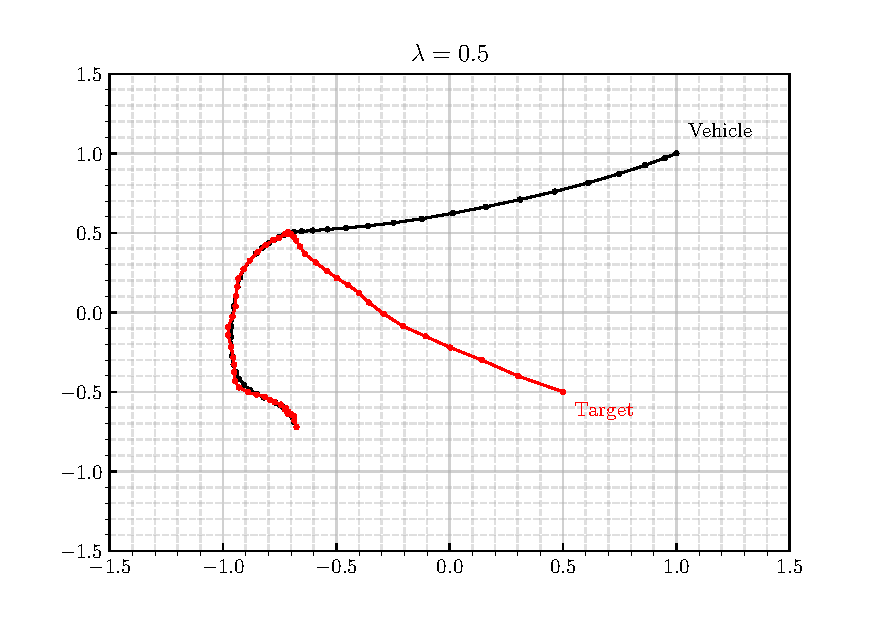
\includegraphics{../../src/task_1/output/ex_1_i=4.pdf}
\end{figure}

\begin{figure}[H]
    \centering
    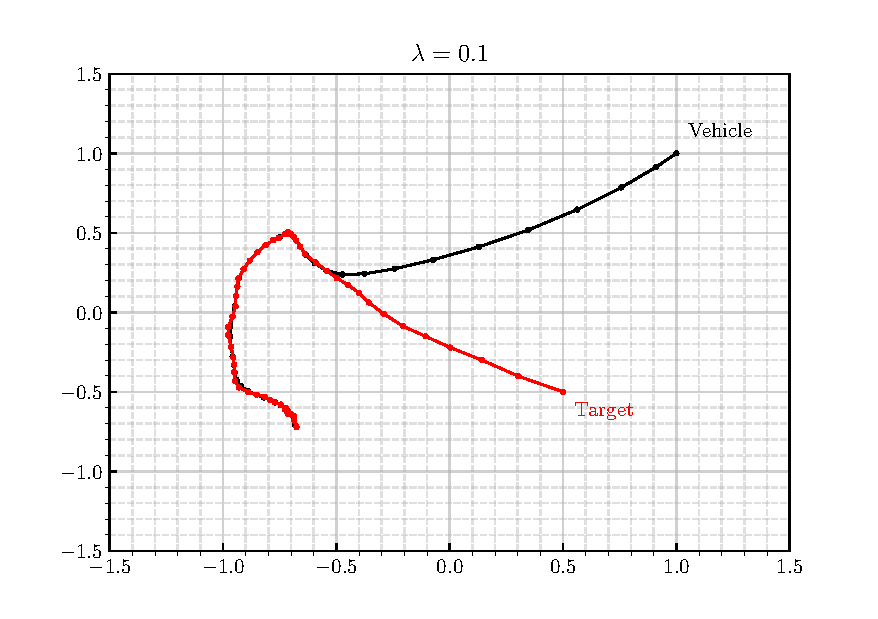
\includegraphics{../../src/task_1/output/ex_1_i=5.pdf}
\end{figure}

\begin{figure}[H]
    \centering
    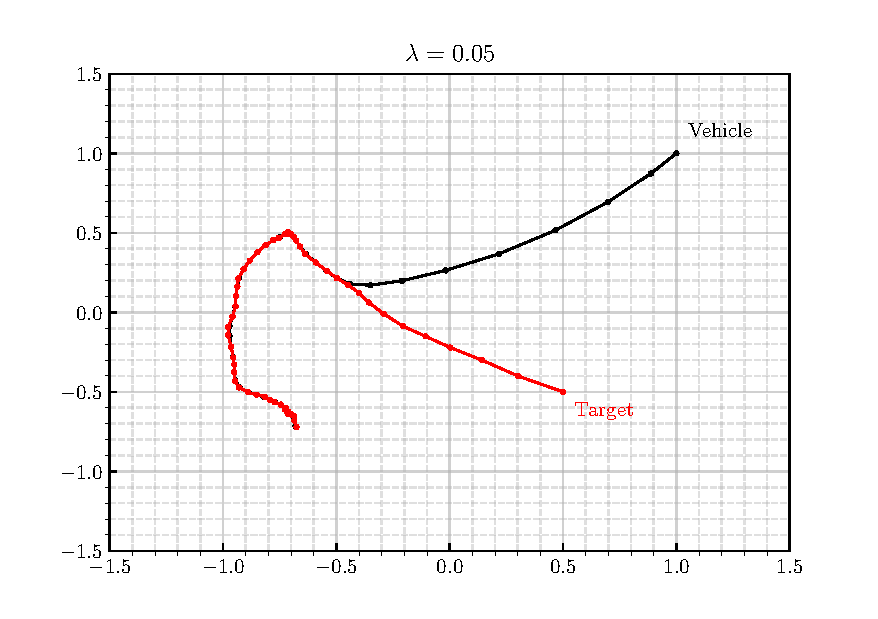
\includegraphics{../../src/task_1/output/ex_1_i=6.pdf}
\end{figure}

\begin{figure}[H]
    \centering
    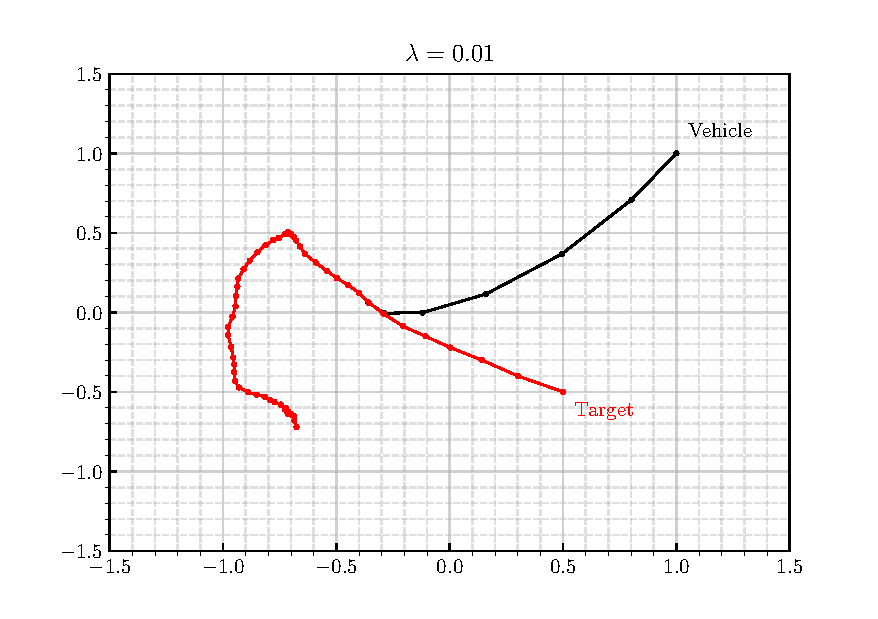
\includegraphics{../../src/task_1/output/ex_1_i=7.pdf}
\end{figure}

\begin{figure}[H]
    \centering
    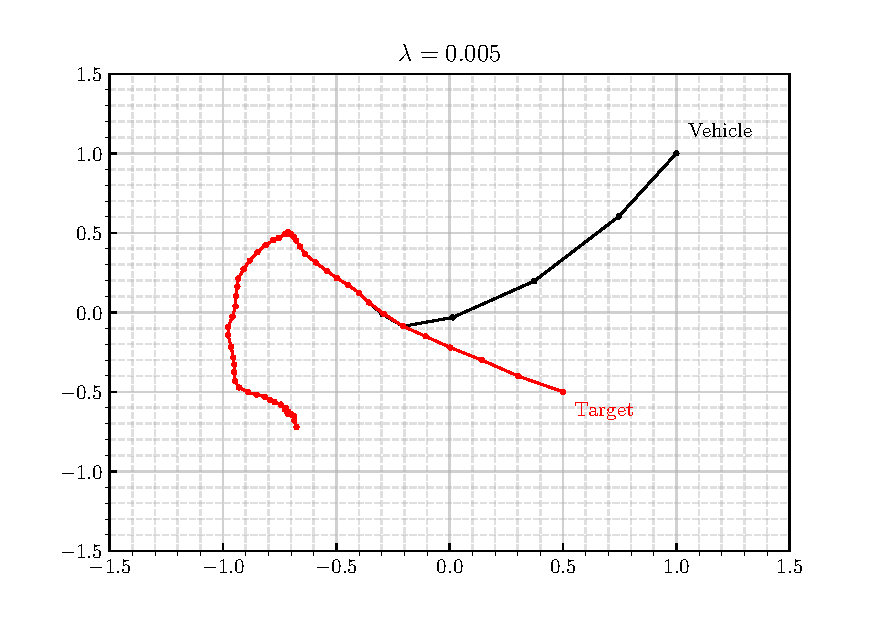
\includegraphics{../../src/task_1/output/ex_1_i=8.pdf}
\end{figure}

\begin{figure}[H]
    \centering
    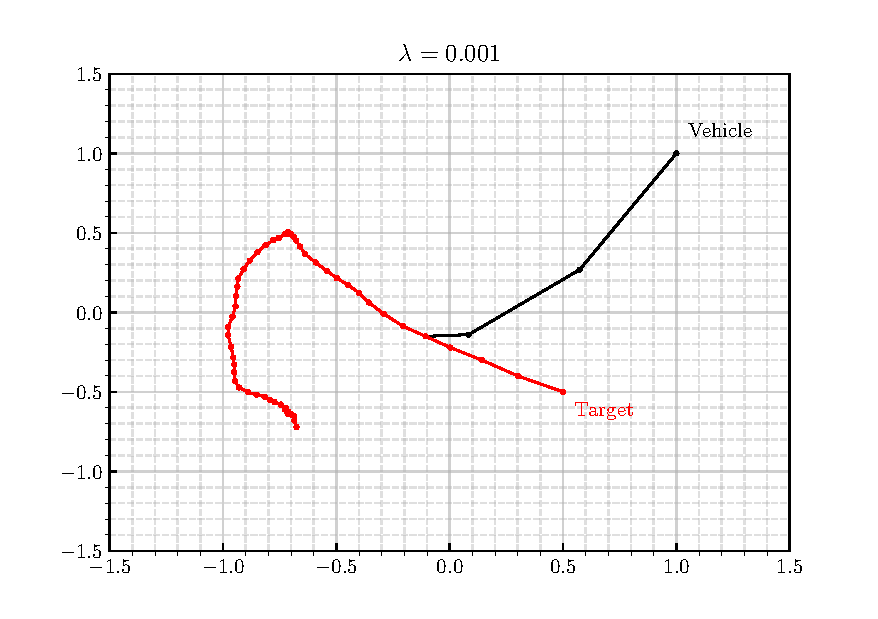
\includegraphics{../../src/task_1/output/ex_1_i=9.pdf}
\end{figure}

\begin{figure}[H]
    \centering
    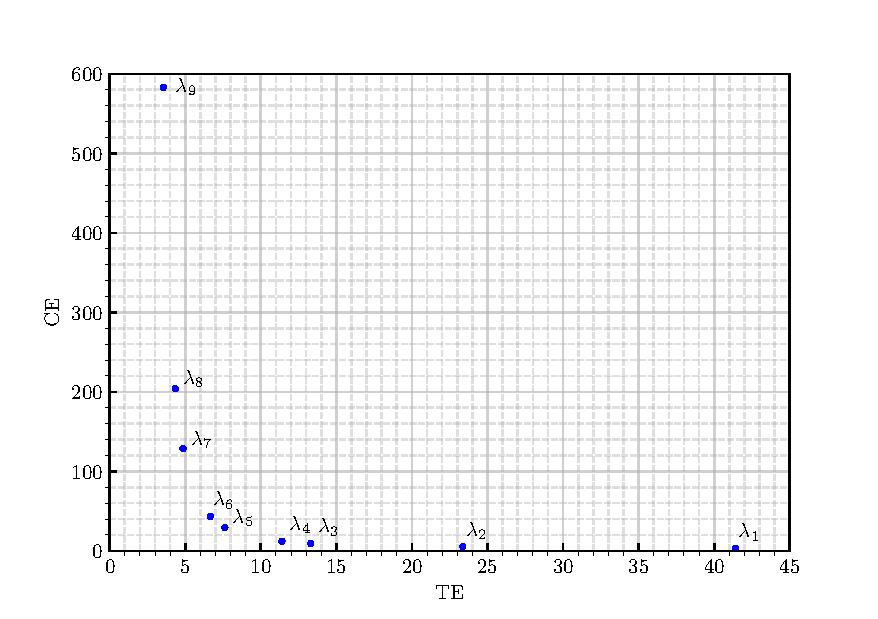
\includegraphics{../../src/task_1/output/TEvsCE.pdf}
\end{figure}

Upon analyzing the plots above, one concludes that a decrease in the parameter $\lambda$ of the optimization problem yields a solution $x^*$ to the correspoding optimization problem such that:
\begin{enumerate}
    \item the resulting vehicle trajectory is overall less dissimilar to that of the target (when it comes to proximity between positions in the two trajectores associated with the same time instant).
    \item the value of the resulting Tracking Effort (TE) decreases, while the corresponding Control Error (CE) registers an increase.
\end{enumerate}
In order to give a rationale for these observations, notice that, for a given value of $(x, u) = (x(1), ..., x(T), u(1), ..., u(T - 1))$, the cost function of the optimization problem can be written as:
\vspace{-0.2em}
\[
    f(x, u) = \text{TE}(x, u) + \lambda \text{CE}(x, u)
\]
As such, we can argue that:
\begin{itemize}
    \item[--] a decrease in $\lambda$ diminishes the importance of the parcel $\lambda \text{CE}(x, u)$ relative to that of $\text{TE}(x, u)$ in the objective function. Hence, bigger decreases in the cost function are more easily attained by lowering the TE instead of the CE, explaining the lower value for the TE that is obtained at an optimal solution. Furthermore, since the parcel TE pertains to the overall proximity of the positions of the target and the vehicle's trajectories at each instant $t$, it also follows that these trajectories tend become similar with the shrinkage of $\lambda$.
    \item[--] Conversely, an increase in $\lambda$ diminishes the importance of the parcel $\text{TE}(x, u)$ relative to that of $\lambda \text{CE}(x, u)$ in the objective function, resulting in a lower value for the CE at an optimal solution, following an analogous reasoning to the one above. Moreover, we have that lower values for the CE result in lower norms for $u$ and, consequently, for $u(t)$ ($t = 1, ..., T-1$). This, together with the relation
    \[
        x(t + 1) = Ax(t) + Bu(t)
    \]
    present in the constraints, explains the fact that changes in the state $x$ also tend to be smaller in norm. Therefore, a lesser degree of similarity between the trajectories is attained, given that the target and the vehicle start at different positions and that the process of reaching the same position at a given instant in time is hindered.
\end{itemize}

\section{Task 2}

\begin{proof}[\unskip\nopunct]
    Let $(x_a, u_a)$ and $(x_b, u_b)$ denote some minimizers obtained after solving the given optimization problem for $\lambda = \lambda_{a}$ and $\lambda = \lambda_{b}$, respectively. Let $\text{TE}(x, u)$ and $\text{CE}(x, u)$ denote the Tracking Error and Control Effort for a given value of $(x, u) = (x(1), ..., x(T), u(1), ..., u(T - 1))$, respectively.
    Then, suppose that $\text{TE}(x_a, u_a) \le \text{TE}(x_b, u_b)$.

    Since $(x_b, u_b)$ minimizes the cost function for $\lambda = \lambda_b$, it follows that:
    \vspace{-0.3em}
    \begin{align}
        \text{TE}(x_b, u_b) + \lambda_b \text{CE}(x_b, u_b) & \le 
        \text{TE}(x_a, u_a) + \lambda_b \text{CE}(x_a, u_a) \\
        & \le \text{TE}(x_b, u_b) + \lambda_b \text{CE}(x_a, u_a)
    \end{align}

    where we used the hypothesis that $\text{TE}(x_a, u_a) \le \text{TE}(x_b, u_b)$ do derive (2) from (1). In particular, we have that:
    \vspace{-0.3em}
    \begin{align*}
        \text{TE}(x_b, u_b) + \lambda_b \text{CE}(x_b, u_b) & \le 
        \text{TE}(x_b, u_b) + \lambda_b \text{CE}(x_a, u_a) \\
        \Leftrightarrow \lambda_b \text{CE}(x_b, u_b) & \le 
        \lambda_b \text{CE}(x_a, u_a) \\
        \Leftrightarrow \text{CE}(x_b, u_b) &\le \text{CE}(x_a, u_a)
    \end{align*}

    with the last inequality coming from the fact that $\lambda_b > 0$. We have thus proven the desired result.
\end{proof}

\section{Task 3}

\begin{proof}[\unskip\nopunct]
To prove that the problem has a unique solution we begin by convert it to an unconstrained optimization problem. By solving the recurrence relation in the constraints we get:
\vspace{-0.1em}
\begin{align*}
    x(t)= Ax(t&-1) + Bu(t-1)
    \Leftrightarrow
    \\
    \Leftrightarrow
    x(t)= A^2x(t&-2) + ABu(t-2) + Bu(t-1)
    \Leftrightarrow
    \\
    \vdots
    \\
    \Leftrightarrow 
    x(t)= A^{(t-1)} & x_{\text{initial}} + \sum_{i=1}^{t-1} A^{(i-1)}Bu(i)
\end{align*}

This closed form can be confirmed using induction in $t$. The induction basis ($t = 1$) is trivially verified (considering that a summation whose lower limit exceeds its upper limit evaluates to zero):
\vspace{-0.8em}
\begin{align*}
    x(1) = A^0 x(1) &= A^0 x_{\text{initial}} +  \sum_{i=1}^{0} A^{(i-1)}Bu(i) \\
    &= A^{(1 - 1)} x_{\text{initial}} +  \sum_{i=1}^{1 - 1} A^{(i-1)}Bu(i)
\end{align*}
\vspace{-0.5em}
For the induction step, we have:
\begin{align*}
    x(t + 1) &= Ax(t) + Bu(t) \\
    &= A \left(  A^{(t-1)} x_{\text{initial}} + \sum_{i=1}^{t-1} A^{(i-1)}Bu(i) \right) + Bu(t) \\ 
    &=  A^{((t + 1)-1)} x_{\text{initial}} + \sum_{i=1}^{t-1} A^{(i + 1 -1)}Bu(i) + Bu(t) \\ 
    &= A^{((t + 1)-1)} x_{\text{initial}} + \sum_{i=2}^{(t + 1)-1} A^{(i-1)}Bu(i) + A^{(1 - 1)}Bu(t) \\ 
    &= A^{((t + 1)-1)} x_{\text{initial}} + \sum_{i=1}^{(t + 1)-1} A^{(i-1)}Bu(i)
\end{align*}
Plugging this into the objective function we now get an unconstrained version of the original problem:
\vspace{-0.5em}
\begin{align*}
    \minimize_{u} \hspace{0.4cm} \underbrace{
    \sum_{t=1}^{T} ||E (A^{(t-1)} x_{\text{initial}} + \sum_{i=1}^{t-1} A^{(i-1)} B u(i)) - q(t)||_{\infty} +
    \lambda \sum_{t=1}^{T-1} ||u(t)||_{2}^2}_{\phi(u)}
\end{align*}

Consider now the following decomposition for the function $\phi$:
\[  
    \phi(u) =  \sum_{t=1}^{T} g_t(u) + h(u)
\]
where 
\vspace{-0.5em}
\begin{align*}
    g_t(u) &= ||E (A^{(t-1)} x_{\text{initial}} + \sum_{i=1}^{t-1} A^{(i-1)} B u(i)) - q(t)||_{\infty} \\
    h(u) &= \lambda \sum_{t=1}^{T-1} \|u(t)\|_{2}^2 = 
    \lambda \left( u_1^2(1)+ u_2^2(1) + ... + u_1^2(T - 1)+ u_2^2(T - 1))\right) \\
    &=  \lambda \|u\|_2^2 = u^T (\lambda I_2) u
\end{align*}

Clearly, $h$ is a strongly convex function, since it is a quadratic function where the matrix associated with the quadratic form present in its expression $(\lambda I_2)$ is positive definite, since all its eigenvalues are $\lambda$ and $\lambda > 0$. \par
On another hand, for $t = 1, ..., T$, $g_t$ can be re-written as:
\begin{align*}
    g_t(u) &= \bigg\|\sum_{i=1}^{t-1} EA^{(i-1)} B u(i) + EA^{(t-1)} x_{\text{initial}} - q(t)\bigg\|_{\infty} \\
    &= \bigg\|
    \underbrace{
    \begin{bmatrix}
        EB & EAB & EA^2B & ... & EA^{(t - 2)}B
    \end{bmatrix}
    }_{\mathcal{A}}
    \begin{bmatrix}
        u(1) \\ u(2) \\ u(3) \\ ... \\ u(T - 1)
    \end{bmatrix}
    + \underbrace{EA^{(t-1)} x_{\text{initial}} - q(t)}_{\beta}\bigg\|_{\infty} \\
    &= \| \mathcal{A}u + \beta \|_{\infty} = (N \circ T)(u)
\end{align*}
where $T(u) = \mathcal{A}u + \beta$ and $N(z) = \|z\|_{\infty}$.\par
Since $N$ is a convex function (it is a norm) and $T$ is an affine map, it follows that $g_t(u)$ is a convex function. Moreover, $\sum_{t=1}^{T} g_t(u)$ is also a convex function, since it is a conic combination of convex functions.
\par
In conclusion, the cost function is the sum of a convex function $(\sum_{t=1}^{T} g_t(u))$ with a strongly convex function ($h(u)$), so it's itself a strongly convex function, thereby proving it has a unique global minimizer and so the optimization problem has a unique solution.
\end{proof}

\section{Task 4}

\begin{figure}[H]
    \centering
    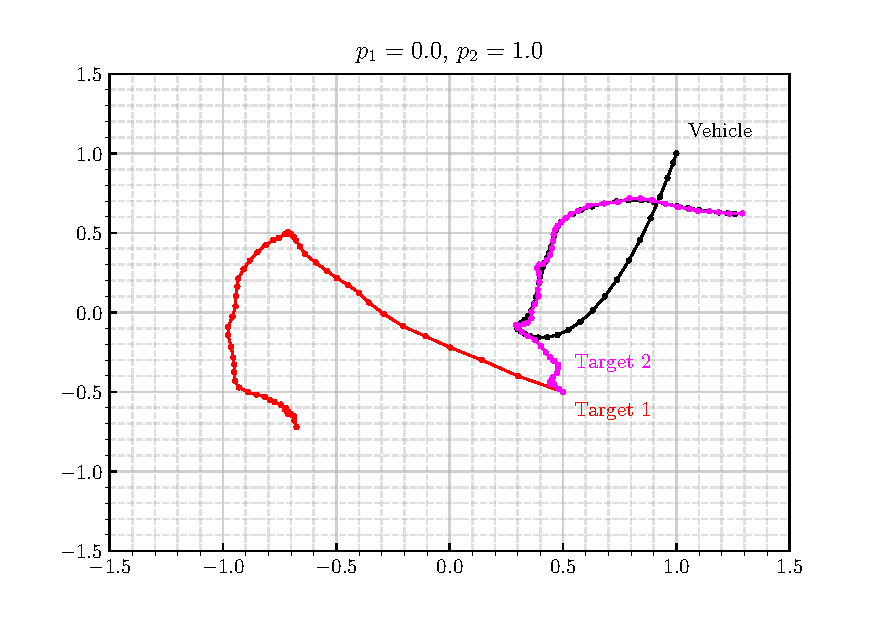
\includegraphics{../../src/task_4/output/ex_4_i=1.pdf}
\end{figure}

\begin{figure}[H]
    \centering
    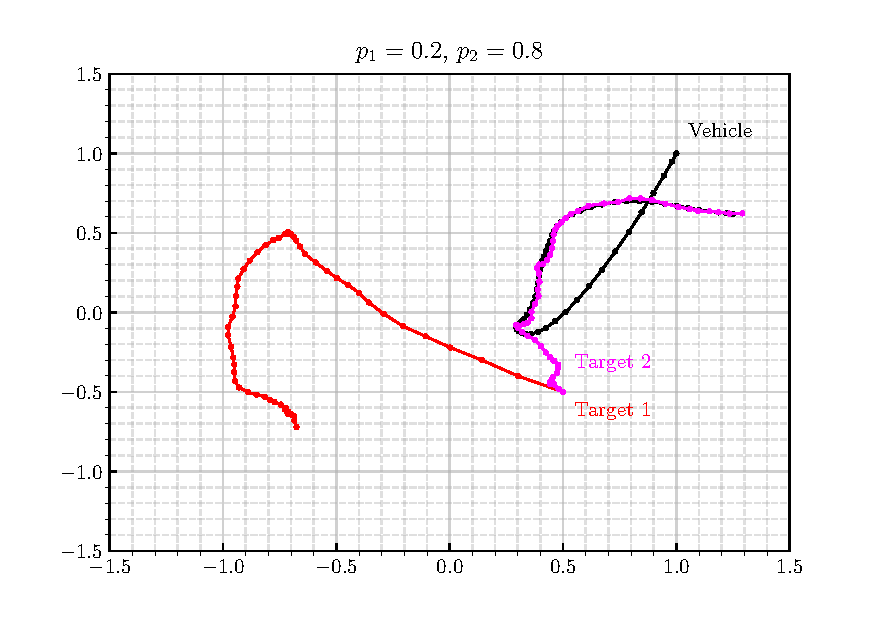
\includegraphics{../../src/task_4/output/ex_4_i=2.pdf}
\end{figure}

\begin{figure}[H]
    \centering
    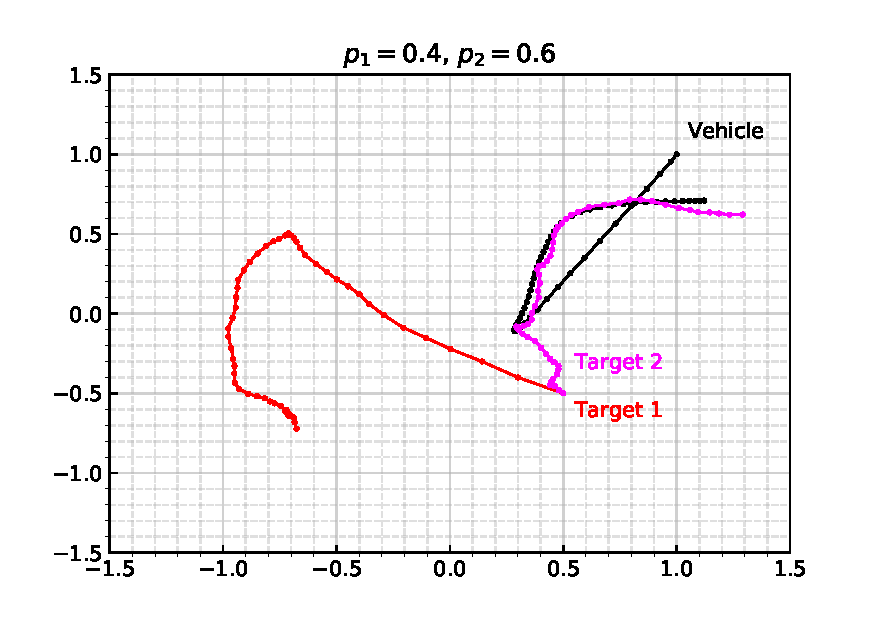
\includegraphics{../../src/task_4/output/ex_4_i=3.pdf}
\end{figure}

\begin{figure}[H]
    \centering
    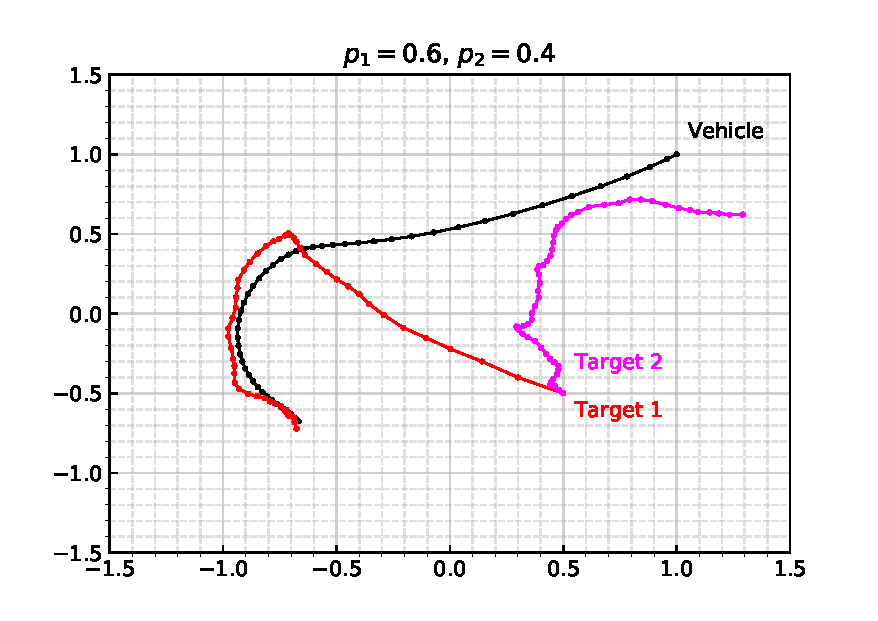
\includegraphics{../../src/task_4/output/ex_4_i=4.pdf}
\end{figure}

\begin{figure}[H]
    \centering
    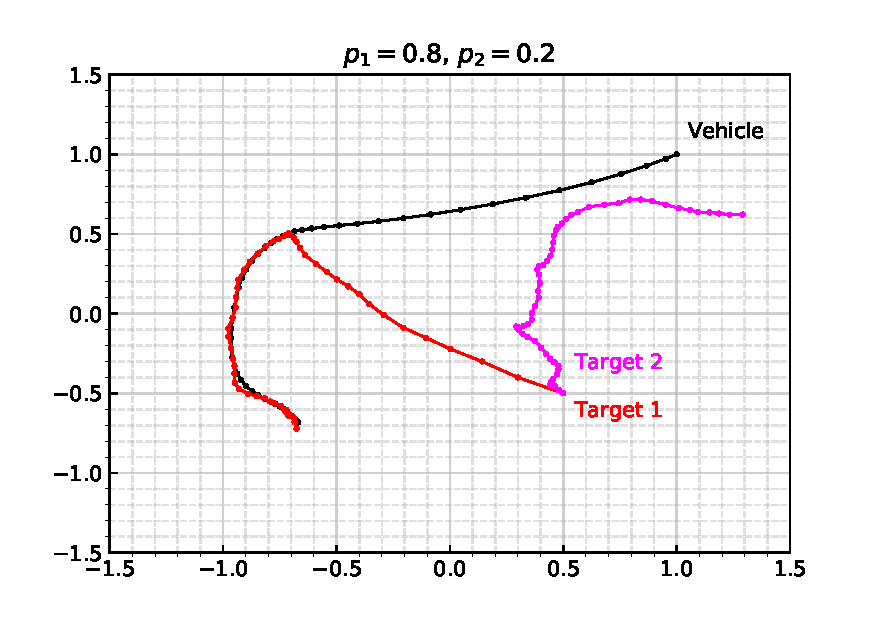
\includegraphics{../../src/task_4/output/ex_4_i=5.pdf}
\end{figure}

\begin{figure}[H]
    \centering
    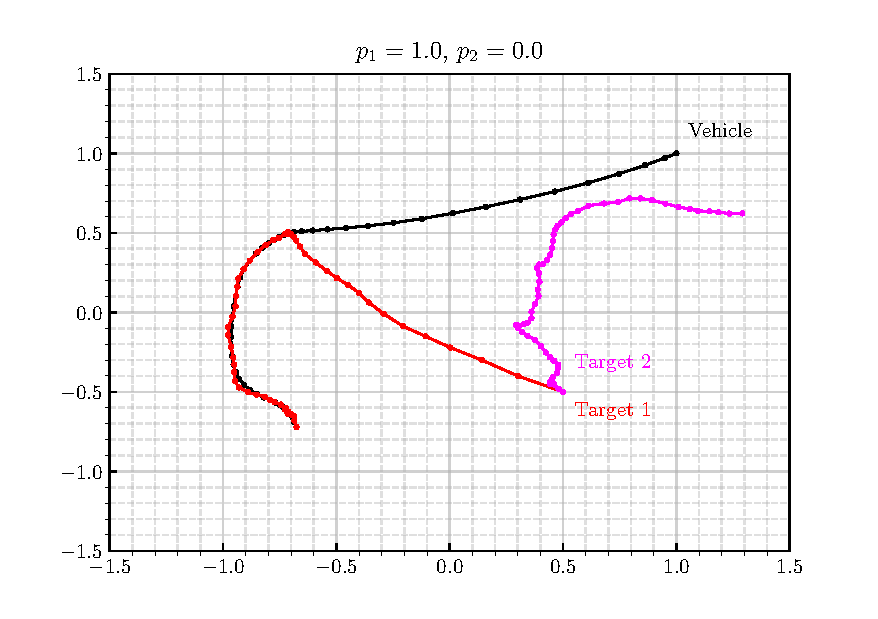
\includegraphics{../../src/task_4/output/ex_4_i=6.pdf}
\end{figure}

%From the results, we can see that the tracker chooses the trajectory with the highest probability. However, if the probability is not 100\%, it is noticeable an "hesitation", the tracker prefers to follow the one with highest probability, but deviated towards the other. \\
From the results, we can see that an increase in $p_i$ yields an increase in proximity to the trajectory of the vehicle $i$ ($i \in \{1, 2\})$ in the sense that, for each time instant, the correspoding position becomes less distant (in this case, according to $l_{\infty}$ distance) to the position of the trajectory of vehicle $i$ in the same instant. Moreover, we observe that this overall proximity is more substantial when it is relative to the trajectory of the vehicle associated with the highest prior probability.

Noting that the cost function can be written as:
\[
    f(x, u) = p_1 \text{TE}_1(x, u) + p_2 \text{TE}_2(x, u) + \lambda \text{CE}(x, u)
\]
we see that, for a fixed lambda, if $p_i$ increases, the parcel $p_i \text{TE}_i(x, u)$ gains more relative importance in the cost function. As such, bigger decreases in the cost function can be more easily attained by lowering $\text{TE}_i(x, u)$. Consequently, the solution $(x^*, u^*)$ yields a lower value of $\text{TE}_i(x^*, u^*)$, and so the resulting trajectory will tend to become overall closer to the one of target $i$. In particular, if $p_i > p_j$, then  $\text{TE}_i(x^*, u^*) >=\text{TE}_j(x^*, u^*)$ and the vehicles trajectory will be more similar to that of vehicle $i$.

\section{Task 5}

Given the current problem formulation, we have that the cost function can be written as:

\[
    f(x_1, u_1, x_2, u_2) = f_1(x_1, u_1) + f_2(x_2, u_2)
\]

where

\[
    f_k(x_k, u_k) = p_k \bigg( \sum_{t=1}^{T} ||Ex_k(t) - q_k(t)||_{\infty} +
    \lambda \sum_{t=1}^{T-1} ||u_k(t)||_{2}^2 \bigg)
\]

with $k \in \{1, 2\}$. Given that the set of constraints can be broken into two sets, each one pertaining to disjoint sets of variables (namely $\{x_1, u_1\}$ and $\{x_2, u_2\}$) and that $p_k \ge 0$ we conclude that $(x_1, u_1)$ and $(x_2, u_2)$ can be obtained by solving two independent optimization problems, each one of the form:
\vspace{-0.5em}
\begin{align*}
    \minimize_{u}& \hspace*{0.4cm} \sum_{t=1}^{T} ||Ex_k(t) - q_k(t)||_{\infty} +
    \lambda \sum_{t=1}^{T-1} ||u_k(t)||_{2}^2 \\
    \text{s.t.}& \;\;\; x_k(1) = x_{\text{initial}} \\ 
    & \;\;\; x_k(t + 1) = Ax_k(t) + Bu_k(t)
\end{align*}

where $k \in \{1, 2\}$. With that being said, we would be obtaining two independent solutions for the problem discussed in Tasks 1, 2 and 3. In turn, these two trajectories would only coincide at the initial instant but would tendentially become closer to the target associated with the correspoding problem. Hence, this formulation is completely agnostic to the fact that, until the target is made known at $t = 35$, the trajectories must be exactly the same.

%The given formulation doesn't include that, until $t = 34$, the tracker will simply follow the minimum cost path between trajectory 1 and 2. Only at $t = 35$ will the tracker follow the true target. Also, there is no coupling between ($x_1$, $u_1$) and ($x_2$, $u_2$). \\

\section{Task 6}

The following constraint solves the questions raised in the previous task: \\
\vspace{-0.3em}
\begin{equation}
    \label{equation_t6}
    u_1(t) = u_{2}(t), \> \> \> 1 \le t \le 34
\end{equation}

Note that $x_1$ and $x_2$ become equal (for $1 \le t \le 34$), given these constraints together with (\ref{equation_t6}): \\
\vspace{-1.6em}
\begin{align*}
    x_1(t+1) = A x_1(t) + B u_1(t), \> \> \> 1 \le t \le T-1 \\
    x_2(t+1) = A x_2(t) + B u_2(t), \> \> \> 1 \le t \le T-1
\end{align*}

\section{Task 7}

\begin{figure}[H]
    \centering
    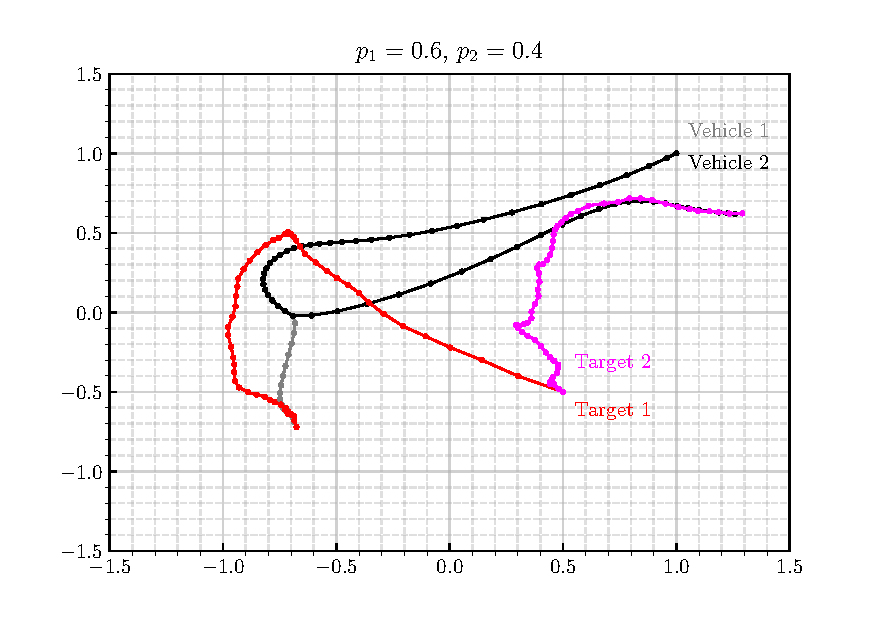
\includegraphics{../../src/tasks_5-7/output/ex_7.pdf}
\end{figure}

\section{Task 8}

Final estimates of $p$ and $v$:

\[
    p^{*} = \begin{bmatrix}1.77002952 \\ -0.92169453
            \end{bmatrix} \; \; \; \; \;
    v^{*} = \begin{bmatrix}-0.95187589 \\ 1.49529891
            \end{bmatrix} 
\]
\vspace{-1em}
\begin{figure}[H]
    \centering
    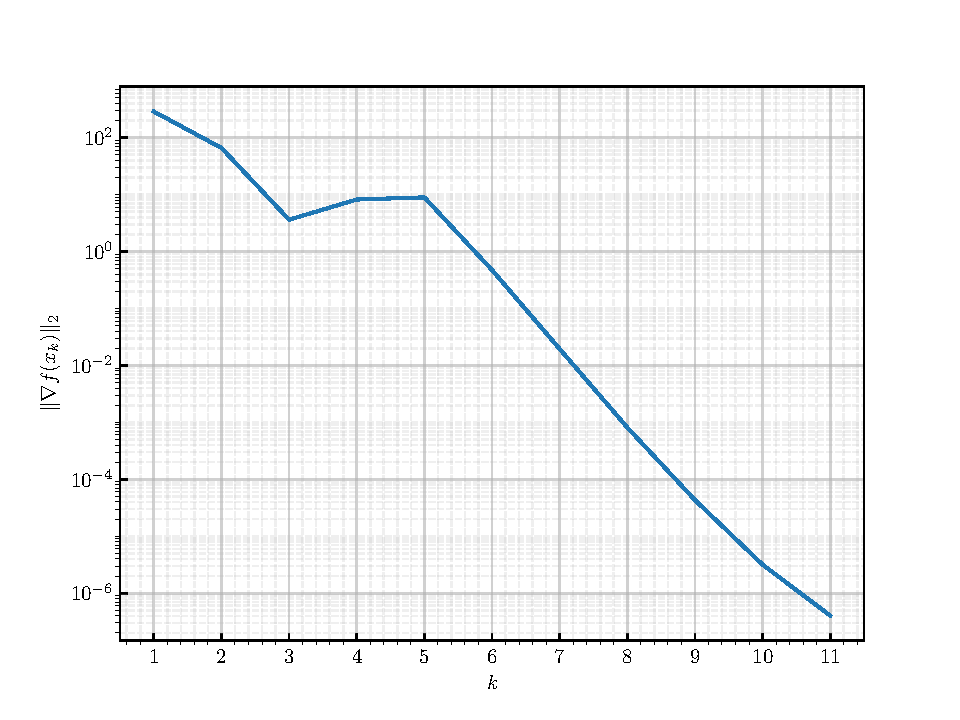
\includegraphics[scale = 0.9]{../../src/task_8/output/gradient_norms.pdf}
\end{figure}
\vspace{-3.3em}
\begin{figure}[H]
    \centering
    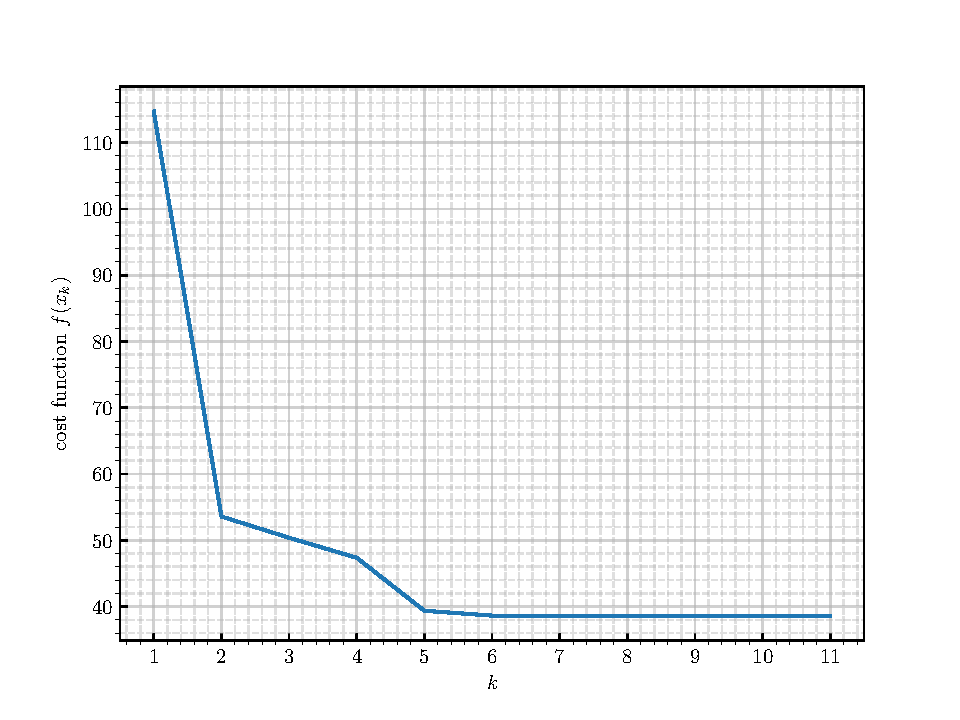
\includegraphics[scale = 0.9]{../../src/task_8/output/cost_function_values.pdf}
\end{figure}
\pagebreak
\subsubsection*{Derivation of the gradients}

In order to apply the Levenberg-Marquardt method, we must write the cost function as a sum of squares of some other functions. To do that, we note that:

\[
    f(p, v) = \sum_{t \in \mathcal{T}} \sum_{i = 1}^2 (g_{t, i}(p, v))^2
\]

where $g_{t, i}(p, v) = \|(p + tv) - s_i \|_2 - r_i(t)$. Since in iteration $(k + 1)$ we solve:

\[
    \minimize_{p, v} \bigg\|A \begin{bmatrix} p \\ v\end{bmatrix} - b \: \bigg\| ^ 2
\]

where

\[
    A = \begin{bmatrix}
        \nabla_{(p, v)}g_{t_1, 1}(p_k, v_k)^T \\
        \nabla_{(p, v)}g_{t_1, 2}(p_k, v_k)^T \\
        ... \\
        \nabla_{(p, v)}g_{t_{|\mathcal{T}|}, 1}(p_k, v_k)^T \\
        \nabla_{(p, v)}g_{t_{|\mathcal{T}|}, 2}(p_k, v_k)^T \\
        \sqrt{\lambda_k} I_4
    \end{bmatrix} \; \; \; \; \; \; 
    b = \begin{bmatrix}
        \nabla_{(p, v)}g_{t_1, 1}(p_k, v_k)^T 
        \begin{bmatrix} p_k, v_k \end{bmatrix}^T - g_{t_1, 1}(p_k, v_k)\\
        \nabla_{(p, v)}g_{t_1, 2}(p_k, v_k)^T 
        \begin{bmatrix} p_k, v_k \end{bmatrix}^T - g_{t_1, 2}(p_k, v_k) \\
        ... \\
        \nabla_{(p, v)}g_{t_{|\mathcal{T}|}, 1}(p_k, v_k)^T 
        \begin{bmatrix} p_k, v_k \end{bmatrix}^T - g_{t_{|\mathcal{T}|}, 1}(p_k, v_k) \\
        \nabla_{(p, v)}g_{t_{|\mathcal{T}|}, 2}(p_k, v_k)^T 
        \begin{bmatrix} p_k, v_k \end{bmatrix}^T - g_{t_{|\mathcal{T}|}, 2}(p_k, v_k) \\
        \sqrt{\lambda_k} [p_k, v_k]^T 
    \end{bmatrix} \; \; \; \; \; \; 
\]

we must compute the gradients $\nabla_{(p, v)}g_{t, i}(p, v)$, for $t \in \mathcal{T}$ and $i \in {1, 2}$. \\
For that purpose, we write $g_{t, i}$ as a composition of functions:
\[
    g_{t, i}(p, v) = h_{t, i}^{(3)}(h_{t, i}^{(2)}(h_{t, i}^{(1)}(p, v)))
\]
where
\begin{align*}
    h_{t, i}^{(1)}(p, v) &= (p + tv) - s_i, \;\;\; p, v \in \mathbb{R}^2 \\
    h_{t, i}^{(2)}(z) &= \|z\|_2, \;\;\; z \in \mathbb{R}^2 \\
    h_{t, i}^{(3)}(u) &= u - r_i(t), \;\;\; u \in \mathbb{R} \\
\end{align*}
and proceed to apply the chain rule:
\begin{align*}
    \nabla_{(p, v)}g_{t, i}(p, v) &= \nabla_{(p, v)}h_{t, i}^{(1)}(p, v) \:
                                    \nabla_{z} h_{t, i}^{(2)}(h_{t, i}^{(1)}(p, v)) \:
                                    \nabla_{u} h_{t, i}^{(3)}(h_{t, i}^{(2)}(h_{t, i}^{(1)}(p, v))) \\
                                  &= \nabla_{(p, v)}((p + tv) - s_i) \:
                                    \nabla_{z} (\|z\|_2)\bigg\rvert_{z = (p + tv) - s_i} \:
                                    \nabla_{u} (u - r_i(t))\bigg\rvert_{u = \|(p + tv) - s_i\|_2} \\
                                  &= \begin{bmatrix} I_2 \\ tI_2 \end{bmatrix} \left( \frac{z}{\|z\|_2}\right)\bigg\rvert_{z = (p + tv) - s_i} \cdot 1 \\
                                  &= \begin{bmatrix} I_2 \\ tI_2 \end{bmatrix} \frac{(p + tv) - s_i}{\|(p + tv) - s_i\|_2}
\end{align*}         

where $I_2$ denotes the $2 \times 2$ identity matrix.
Furthermore, we also have to calculate $\nabla_{(p, v)}f(p, v)$ to evaluate the stopping condition
$\|\nabla_{(p, v)}f(p, v)\| < \epsilon$:

\begin{align*}
    \nabla_{(p, v)}f(p, v) 
    &= \sum_{t \in \mathcal{T}} \sum_{i = 1}^2 \nabla_{(p, v)}(g_{t, i}(p, v))^2 \\
    &= \sum_{t \in \mathcal{T}} \sum_{i = 1}^2 2g_{t, i}(p, v)\nabla_{(p, v)}(g_{t, i}(p, v)) \\
    &= \sum_{t \in \mathcal{T}} \sum_{i = 1}^2 2(\|(p + tv) - s_i \|_2 - r_i(t))
    \begin{bmatrix} I_2 \\ tI_2 \end{bmatrix} \frac{(p + tv) - s_i}{\|(p + tv) - s_i\|_2}
\end{align*}

\appendix  
\clearpage
\addappheadtotoc 
\appendixpage 

\section{Task 1 Code}

\lstinputlisting[language=Python]{../../src/task_1/task_1.py}

\section{Task 4 Code}

\lstinputlisting[language=Python]{../../src/task_4/task_4.py}

\section{Task 7 Code}

\lstinputlisting[language=Python]{../../src/tasks_5-7/task_7.py}

\section{Task 8 Code}

\lstinputlisting[language=Python]{../../src/task_8/task_8.py}

\end{document}
